\documentclass{article}

\usepackage{amsmath}
\usepackage{graphicx}

\newcommand{\rr}{\mathbf{r}}
\newcommand{\ii}{\mathbf{i}}
\newcommand{\jj}{\mathbf{j}}
\newcommand{\kk}{\mathbf{k}}

\DeclareMathOperator{\curl}{curl}

\begin{document}

{\bf Quiz \#13; Tuesday, date: 04/24/2018}

{\bf MATH 53 Multivariable Calculus with Stankova}

{\bf Section \#117; time: 5 -- 6:30 pm}

{\bf GSI name: Kenneth Hung}

{\bf Student name: SOLUTIONS}

\vspace*{0.25in}

\begin{enumerate}
\item Find the area of the part of the paraboloid $z = x^2 + y^2$ that lies within the cylinder $x^2 + y^2 = 1$.

{\em Solution.} We can parametrize the points on here by
\[
x = r \cos \theta, ~~~~ y = r \sin \theta, ~~~~ z = r^2,
\]
where $0 \le r \le 1$ and $0 \le \theta \le 2\pi$. The tangent vectors are
\[
\langle \cos \theta, \sin \theta, 2r \rangle, ~~~~ \langle -r \sin \theta, r \cos \theta, 0 \rangle
\]
and their cross product is
\[
\langle -2r^2 \cos \theta, -2r^2 \sin \theta, r \cos^2 \theta + r \sin^2 \theta\rangle = \langle -2r^2 \cos \theta, -2r^2 \sin \theta, r \rangle.
\]
The surface area is thus
\begin{align*}
\int_0^{2\pi} \int_0^1 \left|\langle -2r^2 \cos \theta, -2r^2 \sin \theta, r \rangle\right| \,dr \,d\theta & = \int_0^{2\pi} \int_0^1 \sqrt{4 r^4 + r^2} \,dr \,d\theta \\
& = \int_0^{2\pi} \,d\theta \int_0^1 r \sqrt{4 r^2 + 1} \,dr \\
& = 2\pi \left[\frac{1}{12} (4r^2 + 1)^{3/2}\right]_0^1 \\
& = \frac{5^{3/2} - 1}{6} \pi.
\end{align*}

\item {\em True / False?} Recall that the integral
\[
\int_C \frac{-y \ii + x \jj}{x^2 + y^2} \cdot d\rr = 2\pi
\]
for any positive oriented simple closed path that encloses the origin. The integral along one loop of the following path is also $2\pi$.
\begin{center}
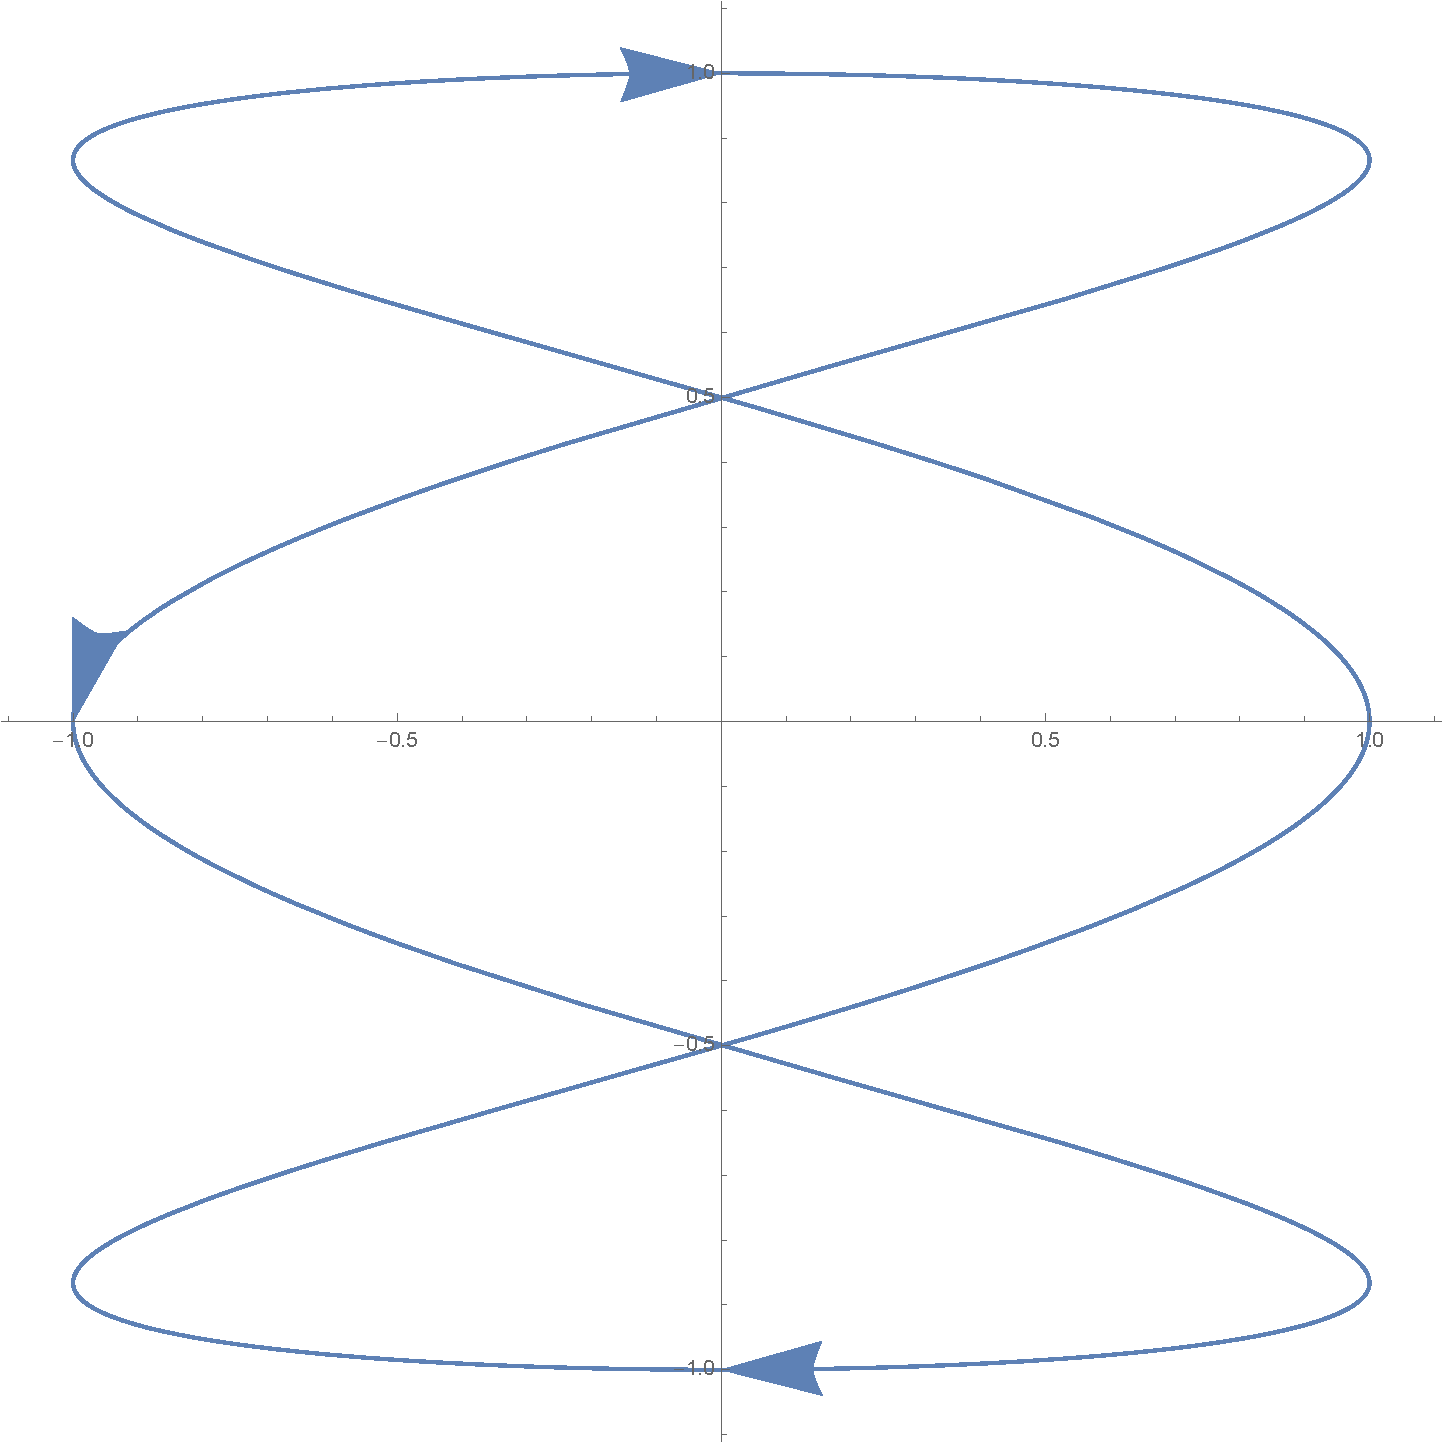
\includegraphics[width=0.5\textwidth]{quiz13dis117pic}
\end{center}

{\em Solution.} {\bf True.} The path can be split into three parts, the upper lobe, the center lobe, and the lower lobe. Only the center lobe of the graph contributes to the integral, and it is counterclockwise, so the integral is $2\pi$.

\item {\em True / False?} For any single functions $f$, $g$, $h$ that are smooth and have continuous derivatives, there is a vector field $\mathbf{G}$ such that $\curl \mathbf{G} = \langle f'(y), g'(z), h'(x) \rangle$.

{\em Solution.} {\bf True.} The divergence of this vector is $0$, so we suspect that it is a curl. By a little bit of trial and error, and noticing the pattern, we find that the curl of $\langle g(z), h(x), f(y) \rangle$ gives that.
\end{enumerate}

\end{document}